
Laskuvarjon lentämisen päätarkoituksena on tuoda hyppääjä ehjänä alas. Riippumatta siitä, mitä laskeutumistekniikkaa käytät, ensisijaiset tavoitteesi pysty- ja vaakavauhdin loppuessa ovat seuraavat: 

\begin{enumerate}[label=\bfseries \arabic*)]
\item  \textbf{Vauhdin pysähtymisen pitää tapahtua turvallisella korkeudella maasta} (ei maan sisällä tai 10 m korkeudella) 
\item  \textbf{Kuvun tulee olla vaakalennossa pään päällä} (varjo ei ole kaarroksessa, syöksyssä tai sakkauksessa) 
\item  \textbf{Laskeutuminen tapahtuu vastatuuleen} (kuitenkin mieluummin myötä- tai sivutuuleen kuin kohtia 1 tai 2 rikkoen) 
\end{enumerate}

Opettele tarvittaessa sanomaan ei vauhditetuille laskeutumisille: 

\begin{itemize}
\item  kun ilmassa tai laskeutumisalueella on paljon muuta liikennettä 
\item  laskeutuessasi vieraaseen paikkaan 
\item  sääolosuhteiden ollessa marginaaliset (puuskainen tuuli, turbulenttinen keli) 
\item  ollessasi väsynyt, vihainen tai tyytymätön suoritukseesi vapaapudotuksessa.  
\end{itemize}

Muistuta itseäsi, että voit tehdä vauhdikkaan laskun myös jollakin tulevalla hypyllä, kun olosuhteet ovat paremmat. Se onnistuu kuitenkin vain selviämällä hengissä tästä hypystä.  

\section{ Suora finaali ilman vauhdinottoa }
\label{laskeutumistekniikat-suora-finaali-ilman-vauhdinottoa}


Suora finaali ilman vauhdinottoa on perustapa laskeutua. Tässä laskeutumistekniikassa viimeisestä käännöksestä ennen loppuvetoa on kulunut niin paljon aikaa, että siitä aiheutuneesta nopeuden lisääntymisestä ei ole mitään jäljellä ennen loppuvedon aloittamista. Kaikilla nykyaikaisilla kuvuilla voidaan laskeutua ilman vauhdinottoa, jos käytettävä siipikuorma on järkevä kyseiselle varjolle. Mikäli sinusta tuntuu, että vauhdinotto on tarpeen kunnollista laskeutumista varten, laskeutumistekniikkasi on virheellinen. Jos sinulla on toistuvasti vaikeuksia laskeutua suoralla finaalilla, ei ole turvallista aloittaa vauhditettujen laskeutumisten harjoittelua.  


Vaikka osaisit peruslaskeutumistekniikan, eivätkä sinua kiinnosta nopeat laskeutumiset, on silti hyvä opetella pienen lisävauhdin vaikutus laskeutumiseen. Näin olet paremmin varautunut, jos laskeutumisnopeutesi on jostain syystä tavallista suurempi. Näin voi olla esimerkiksi joutuessasi laskeutumaan myötätuuleen tai väistämään toista varjoa matalalla. Kannattaa myös harjoitella loivia kaarroksia fleerin aikana, jotta osaat väistää mahdollisia esteitä. Tätä harjoittelua varten saatat myös tarvita hieman lisävauhtia. 

\section{ Suora vauhditus etummaisista kantohihnoista }
\label{laskeutumistekniikat-suora-vauhditus-etummaisista-kantohihnoista}


Ennen kuin harjoittelet etummaisista kantohihnoista vauhditettuja lähestymisiä, varmista, että ohjauspunoksesi ovat riittävän pitkät ja että kantohihnoissasi on lenkit tarttumista varten. Oikean mittaisissa ohjauspunoksissa on muutama sentti löysää täysliidossa ja punokset muodostavat loivan kaaren matkalla takahelmasta ohjauslenkkiin.  


Jos ohjauspunokset ovat liian lyhyet, vedät myös kuvun takareunaa alas vetäessäsi kantohihnoista. Tämä saattaa aiheuttaa kuvun nyökkimistä tai muuta epävakautta. Jos varjo jossain tilanteessa vaikuttaa epävakaalta, lopeta kokeilu. Pidä aina kiinni ohjauslenkeistä, kun käytät kantohihnoja ohjaamiseen tai vauhdin lisäämiseen. Toisen tai molempien ohjauslenkkien luiskahtaminen pois kädestä lähellä maata kesken vauhdinoton on erittäin vaarallista. Harjoittele aluksi korkealla kaikkia asioita, joita aiot myöhemmin kokeilla lähellä maata. 


Turvallisin tapa lisätä laskeutumisvauhtia ja pidentää fleerin pituutta on käyttää suoraa lähestymistä ja lisätä varjon nopeutta vetämällä alas molemmista etummaisista kantohihnoista. Vaadittavan vedon määrä riippuu varjotyypistä mutta on yleensä noin 5 - 10 cm. Kun molempia kantohihnoja vedetään alas, painopiste kuvun alla siirtyy taaksepäin, varjon liitokulma jyrkkenee ja vajoamisnopeus kasvaa. Näin saadaan lisää vauhtia, joka muuttuu nosteeksi loppuvedossa. Veto kantohihnoista kannattaa vapauttaa rauhallisesti eikä yhtäkkiä päästäen, sillä näin kuvun aerodynaamiset ominaisuudet toimivat parhaiten. Kun päästät kantohihnat vapaaksi oikealla korkeudella, varjo alkaa fleerata itsestään painopisteen siirtyessä eteenpäin ja liitokulman samalla loiventuessa. Jos päästät kantohihnat korkeudella, josta sinun on välittömästi aloitettava loppuvedon tekeminen, olet päästänyt irti liian matalalla. 

\section{ Vauhdin ottaminen etummaisista kantohihnoista kääntämällä }
\label{laskeutumistekniikat-vauhdin-ottaminen-etummaisista-kantohihnoista-kaantamalla}


Lisävauhdin hakeminen käännöksellä on aina vaarallista, koska varjon vajoamisnopeus kasvaa huomattavasti, vajoamisen pysäyttäminen nopeasti on vaikeaa etkä välttämättä näe kaikkea muuta liikennettä. Harjoittele etummaisista kääntämistä ensin korkealla ja tarkkaile, miten niistä vetäminen vaikuttaa ilmanopeuteen, vajoamiseen ja varjon käyttäytymiseen ylipäänsä. Liian paljon vetäminen voi tukahduttaa reunatunneleita ja on erittäin vaarallista matalalla.  


Laskeutumista varten suoritettava vauhdinotto on aina aloitettava riittävän korkealla oikaisua varten ja se on pystyttävä aina keskeyttämään tarvittaessa. Tämän vuoksi koko käännössektorin on oltava vapaa esteistä ja mahdollistettava laskeutuminen koko sektorille. Jos vauhdinoton aikana näyttää siltä, että korkeus loppuu kesken, älä koskaan jyrkennä kaartoa päästäksesi vastatuuleen, vaan jätä vauhdinotto kesken ja laskeudu sivutuuleen tai käännä varjoa fleerin aikana. Tässä vaiheessa sinun pitää osata nämä tekniikat. Jos et osaa, lopeta vauhdinottoharjoitukset ja keskity ensin perusasioihin. 


Etummaisesta kantohihnasta vedettäessä kuvun kyseisen puolen liitokulma jyrkkenee ja kuvun alla oleva painopiste heilahtaa vastakkaiselle puolelle, mikä aiheuttaa varjon kääntymisen vedon puoleiseen suuntaan. Tällöin vajoamisnopeus kasvaa. Vajoamisnopeuden ja ilmanopeuden kasvaessa kantohihnaan kohdistuu yhä enemmän kasvavan nosteen aiheuttamaa voimaa ja vetäminen käy raskaaksi. Liian paljon vedettäessä tai turbulenttisella kelillä voi aiheutua vakava vajaatoiminta, jos ilmavirran kohtauskulma muuttuu negatiiviseksi ja kuvun kulma kääntyy alakautta ympäri. 


Parhaiten ja turvallisimmin etummaiskäännöksellä saa vauhtia tekemällä laajan, loivan kaarroksen, jossa vauhti kasvaa vähitellen. Tällöin on myös aina mahdollista lopettaa vauhdinotto ja palata nopeasti vaakalentoon, jos korkeus alkaa käydä vähiin. Aloita harjoittelu loivalla 30 - 45 asteen käännöksellä ja etene jyrkempiin käännöksiin vasta, kun osaat ajoittaa ja suorittaa loivan käännöksen tarkasti ja turvallisesti. Jos joudut ohjauslenkeistä nopeasti vetämällä pysäyttämään vajoamisen, olet suorittanut vauhdinoton aivan liian matalalla. Ole aina valmis pelastamaan tilanne oikaisemalla ohjauslenkeillä, jos käännös näyttää menevän matalaksi. 


Nopeasti suoritetut jyrkät heilahtavat käännökset ovat erityisen vaarallisia, koska ilmatilan tarkkailu on niissä vaikeaa ja varjon takaisin vaakalentoon saaminen vaatii huomattavasti enemmän aikaa ja korkeutta kuin kaartaen tehdyssä käännöksessä. Kun olet tehnyt nopean käännöksen, menee huomattavasti aikaa ja korkeutta ennen kuin saat varjon taas täysin takaisin hallintaasi. Yli 180 asteen käännökset ovat äärimmäisen vaarallisia. 


\begin{Figure}\centering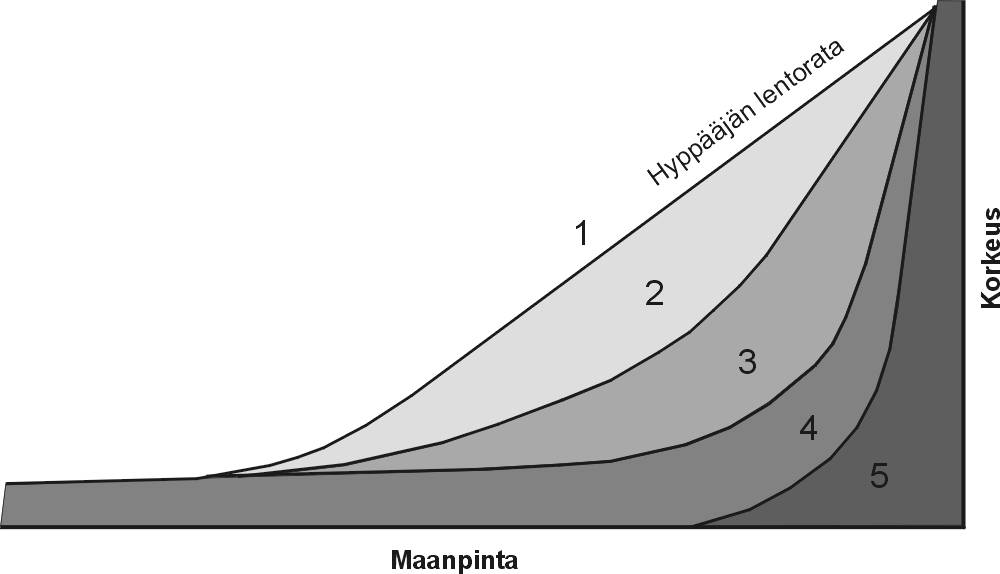
\includegraphics[width=0.99\textwidth]{Lentoradat.jpeg}\captionof{figure}{Hyppääjän lentorata erilaisissa lähestymistekniikoissa}\end{Figure}  

\begin{enumerate}[label=\bfseries \arabic*)]
\item  Suora lähestyminen ja normaali loppuveto. Turvallisin tapa laskeutua. 
\item  Suora lähestyminen molemmilla etukantohihnoilla tai laajalla etukantohihnoista tehdyllä kaarroksella vauhdittaen. Varjo alkaa fleerata itsestään, jos etukantohihnat päästetään riittävällä korkeudella. Suhteellisen turvallista, riskinä vaakanopeuden kasvu.  
\item  Jyrkkä käännös matalalla kantohihnoista tai jarruista. Varjo oikenee vain jarruja käyttäen. \textbf{Riski virheeseen kasvaa huomattavasti.} 
\item  Liian matala tai jyrkkä käännös kantohihnoista tai jarruista nurkassa. Varjon saattaminen vaakalentoon voi olla mahdotonta. \textbf{Onnettomuusvaara} 
\item  Liian matala käännös kantohihnoista tai jarruista. Varjon saaminen vaakalentoon mahdotonta. \textbf{Onnettomuus} 
\end{enumerate}

Erilaiset varjot vaativat erilaisia edistyneitä tekniikoita optimaalisen vauhdin saamiseksi. Tällaisia ovat mm. vauhdinoton aloitus ensin molemmista kantohihnoista vetämällä ja sen jälkeen molemmista kantohihnoista kääntämällä tai käyttämällä valjaskäännöksiä. Opettele korkealla, kuinka varjosi reagoi eri tapoihin.  

\section{ Ohjauslenkeistä tehty käännös vauhdin saamiseksi }
\label{laskeutumistekniikat-ohjauslenkeista-tehty-kaannos-vauhdin-saamiseksi}


\textbf{Älä tee tätä.} Ohjauslenkeistä matalalla tehdyt käännökset ovat hengenvaarallisia riippumatta siitä, ovatko ne tahallaan vai vahingossa tehtyjä. Ne ovat vielä vaarallisempia kuin etummaisista tehdyt nopeat käännökset, koska tällöin jo käännöstä tehtäessä käytetään sitä ohjauspintaa, jolla käännös tarvittaessa keskeytetään ja varjo oikaistaan vaakalentoon käännöksen tapahduttua liian matalalla. Näin ollen oikaisu voi olla täysin mahdotonta ennen törmäystä. Kaikilla kuvuilla saa paremmin ja turvallisemmin pitkiä fleerejä etummaisilla kantohinnoilla suoritetuilla vauhdinotoilla. 

\section{ Loppuvedon tekeminen takimmaisia kantohihnoja käyttäen }
\label{laskeutumistekniikat-loppuvedon-tekeminen-takimmaisia-kantohihnoja-kayttaen}


Loppuvedon, tai osan siitä, voi tehdä myös takimmaisia kantohihnoja käyttäen. Jos ohjauspunos katkeaa/jumittuu tai ohjauslenkki irtoaa korkeudella, jossa varavarjotoimenpiteitä ei kannata enää tehdä, voi loppuvedon suorittaa takimmaisista kantohihnoista vetämällä. Loppuvedon tekemistä ja varjon ohjaamista takimmaisista muutenkin kannattaa harjoitella aluksi korkealla kokeillen, miten varjo reagoi. Varjo reagoi takimmaisista käännettäessä herkästi verrattuna ohjauslenkkeihin, koska tällöin ohjaamiseen käytetään ¼ varjon pinta-alasta. Molemmista kantohihnoista vedettäessä varjo saattaa sakata varsin herkästi ja yllättäen. Kannattaa siis kokeilla jo korkealla, kuinka paljon niistä voit vetää. Jos joudut hätätilanteessa tekemään loppuvedon takimmaisista, ole valmiina kierähtämään. 


Erittäin nopeilla ja kisavarjoilla voidaan fleeri vauhdinoton jälkeen aloittaa käyttämällä takimmaisia kantohihnoja ja tehdä vasta loppujarrutus ohjauslenkeillä. Tämä tekniikka pienentää kuvun vauhtia fleerissä vähemmän, kun varjon takareunaa ei aluksi käännetä lainkaan, vaan vaikutetaan vain kuvun liitokulmaan. Vasta kun vauhti on hidastunut niin, että takimmaisista vetäen/levittäen ei ole mahdollista lisätä nostetta, tehdään loppujarrutus ohjauslenkeillä. Tämä tekniikka on erittäin vaativa ja sitä tulee harjoitella erittäin paljon (kymmeniä kertoja) korkealla ennen sen käyttämistä laskeutumiseen, koska varjo sakkaa takimmaisista kantohihnoista hyvin helposti. Näissä vauhdeissa epäsymmetrisen vedon aiheuttama nopea kääntyminen lähellä maata voi olla kohtalokasta. Tekniikka kannattaa harjoitella jo luokan 4 varjoilla, eikä vasta erittäin suurella siipikuormalla lentäen. Älä siis yritä tätä ilman satojen nopeiden laskeutumisten tuomaa kokemusta.  

\section{ Jarrulasku }
\label{laskeutumistekniikat-jarrulasku}


On tilanteita, joissa on välttämätöntä suorittaa loppuveto osittaisesta jarrutustilasta. Jos joudut käyttämään varalaskeutumispaikkaa pää- tai varavarjolla, on aina mahdollisuus siihen, että käytettävissäsi oleva laskeutumisalue on huomattavasti pienempi kuin mihin olet tottunut. Tällöin on ehkä pakko suorittaa loppuveto jarrutustilasta. Jarruilta tehtävässä loppuvedossa on huomattavasti vähemmän energiaa muutettavissa nosteeksi kuin täydestä liidosta tehtävässä. Toisaalta, kun tehdään loppuveto jarruilta, voidaan minimoida varjon eteenpäin kulkema matka fleerin aikana. Lisäksi lähestymiskulma on jyrkempi. Tämän vuoksi loppuvedon on tapahduttava varsin alhaalla ja ripeästi. Jos joudut laskeutumaan erittäin ahtaaseen paikkaan voimakasta jarrutusta käyttäen, varaudu kierähtämään. Se estää yleensä loukkaantumiset. 


Muista, että tuulisella ilmalla esim. pienelle metsäaukiolle tai muuten korkeiden esteiden reunustamalle alueelle laskeutuessasi saatat kohdata voimakasta turbulenssia esim. puiden latvuston korkeudella. Jos lennät liian suurilla jarruilla, voi turbulenssi tukahduttaa varjosi. Tämän turbulenssikerroksen alapuolella taas saattaa olla hyvinkin tyyntä. Jarrulaskeutumisia kannattaa harjoitella, koska niitä joutuu tekemään varsin harvoin, eikä niitä korkealla siipikuormalla ole kovinkaan helppoa tehdä. Pakkotilanteen tullessa on hyvä tietää, että jarrulaskeutuminen varmasti onnistuu. 

\section{ Jarrukäännös }
\label{laskeutumistekniikat-jarrukaannos}


Jos joudut laskeutumisessasi turvautumaan jarrukäännökseen, on yleensä omassa (tai jonkun toisen) varjolla lentämisessä aiemmin mennyt pieleen monta asiaa. Ilmatilan, korkeuden tai sijainnin tarkkailu tai laskeutumiskuvion suunnittelu ovat todennäköisesti olleet puutteellisia. Voit myös joutua alhaalla väistämään jotakuta muuta, joka on tehnyt nämä virheet. Jarrukäännöksessä on tarkoitus kääntää lentosuuntaa 90 – 180 astetta suhteellisen matalalla. Käännöksen pitää tällöin päättyä suoraan loppuvetotilanteeseen. Jarrukäännöksessä aloitetaan käännös ensin toisella ohjauslenkillä. Samalla aloitetaan vauhdin jarruttaminen myös vastakkaisella ohjauslenkillä, kuitenkin niin, että käännös jatkuu aina haluttuun suuntaan asti. Kun ollaan halutussa suunnassa, ovat molemmat ohjauslenkit alhaalla täysjarrutustilassa ja varjo fleeraa vauhdin pois lähellä maanpintaa.  


Tämä laskeutumistapa on vaarallinen, mutta joskus sitä voidaan käyttää vielä vaarallisemman tilanteen välttämiseksi. Esimerkiksi toiseen varjoon törmääminen matalalla tai laskeutuminen käynnissä olevaa ilma-alusta päin voivat olla tällaisia tilanteita. Harjoittele jarrukäännöstä korkealla ilmassa ja huomioi aina, kuinka paljon/vähän korkeutta menetät 90° tai 180° jarrutetussa käännöksessä niin, että lopussa olet täysjarrutustilassa. Näin tiedät, miltä korkeudelta saatat pakollisessa väistössä onnistua pienimmin mahdollisin vaurioin. 

\section{ Sivu- ja myötätuulilaskut }
\label{laskeutumistekniikat-sivu-ja-myotatuulilaskut}


Joissain tilanteissa voit joutua laskeutumaan sivu- tai myötätuuleen. Tilanne voi tulla täysin tarkoituksellisesti laskeutumisalueen asettamien vaatimusten vuoksi tai yllättäen, jos vastatuuleen kääntyminen ei ole enää mahdollista korkeuden tai muun laskeutuvan liikenteen vuoksi. Tämän vuoksi olisi hyvä harjoitella sivu- ja myötätuulilaskuja etukäteen. Harjoittelu poistaa myös selkärankaan iskostunutta tarvetta laskeutua aina vastatuuleen, mikä nopeana tilanteena matalalla saattaa olla hengenvaarallinen päätös. Myötätuulilaskusta selviää aina pienemmin vahingoin kuin matalalla tehdystä käännöksestä ja maahan iskeytymisestä. Harjoittele kumpaakin kuitenkin verraten heikkoon ja tasaiseen tuuleen; tarkoituksella ei kannata rikkoa itseään. 


Myötätuulilaskun suorittamisessa tärkeää on fleerin ajoittaminen ja valmius kierähtämiseen, jos vauhtia on lopuksi liikaa. Fleeri pitää aloittaa oikeassa korkeudessa, usein hieman korkeammalla kuin vastatuuleen tehtäessä, ja se pitää saattaa loppuun juuri jalkojen ollessa maanpinnan tasolla. Jos olet puolentoista metrin korkeudessa, kun varjosta loppuu kanto, ja vaakavauhtia on vielä runsaasti jäljellä tuulen vuoksi, tulee laskusta varmasti kova. Toisaalta, jos myötätuulta on paljon, voi onnistuneenkin fleerin jälkeen vaakavauhtia olla liikaa pois juostavaksi. Valmistaudu siis aina kierähtämään. Älä ota käsillä vastaan, sillä myötätuulilaskuissa yleisimpiä vammoja ovat rannevammat. 


Sivutuulilaskut kannattaa opetella myös etukäteen. Sivutuulilaskussa normaalilla fleeri-tekniikalla (ohjauslenkit samalla tasolla) varjo alkaa liukua myötätuuleen ja hyppääjä yrittää ottaa tukea tuulen puoleisella jalalla/kädellä kääntäen samalla varjoa lisää. Lopulta hyppääjä kaatuu myötätuulen puolelle (tasapainoansa, suojautumisansa; ks. luku 10). Sivutuulilaskussa pitääkin varjoa kääntää fleerin aikana hiukan vastatuulta kohti, jolloin hyppääjä liikkuu suoraan suhteessa maahan. Kääntäminen suoritetaan vetämällä hieman enemmän tuulen puoleista ohjauslenkkiä; epäsymmetrisyyden määrä riippuu tietenkin varjosta, tuulen nopeudesta, jne. Vasta lopuksi voi vetää toisenkin lenkin pohjaan, jos siihen on tarvetta. 

\section{ Oikeaoppinen loppuveto }
\label{laskeutumistekniikat-oikeaoppinen-loppuveto}


Loppuvedon tarkoitus on muuttaa alaspäin suuntautuvan vauhdin ja liike-energian suunta eteenpäin meneväksi. Oikeaoppinen loppuveto aloitetaan terävällä alkuvedolla vetämällä ohjauslenkit noin olkapäiden korkeudelle. Tarvittava terävyys ja määrä riippuvat varjon ominaisuuksista. Tällöin hyppääjän paino siirtyy kuvun alla eteenpäin, varjon liikesuunta muuttuu ja se alkaa lentää vaakalentoa. Korkeus pidetään vetoa lisäämällä, jolloin myös vauhti hidastuu. 


\begin{Figure}\centering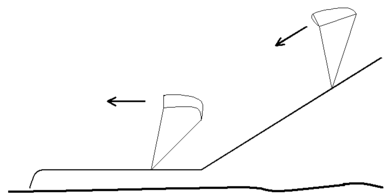
\includegraphics[width=0.9\textwidth]{Oikeaoppinenloppuveto.png}\captionof{figure}{Varjon liikesuunnan muuttuminen tehokkaasti suoritetussa loppuvedossa}\end{Figure} 


Oikein suoritetussa fleerissä ohjauslenkit ovat vaakalennon aikana noin puolijarrutustilassa ja siten hyppääjällä on ohjauksen suhteen pelivaraa. Varjoa tuleekin aktiivisesti lentää niin kauan, että sen ilmanopeus loppuu. Ohjaa varjoa pienin, tasaisin liikkein. Näin varjo lentää paremmin ja sen vakauttaminen turbulenssissa on helpompaa. Myös muiden on helpompi ennakoida mitä teet. 


Siipikuorman pienentäminen, vastatuulen kasvaminen ja varjon suurempi lentonopeus pienentävät kukin tarvittavan loppuvedon terävyyttä ja syvyyttä jopa niin, että loppuveto voi olla hidas ja rauhallinen. Vauhditetuissa laskeutumisessa loppuvedon voi aloittaa korkeammalla ja rauhallisemmin, koska energiaa on fleerin aikana muutettavissa nosteeksi sitä enemmän, mitä enemmän vauhtia on. 

